\subsection{Machine Learning}

\begin{flushleft}
ML Algorithm Overview
\begin{tabularx}{\textwidth}{p{6.5em}|p{7.7em}|p{9.5em}|X}
\hline
\rowcolor{gray!30}
Variable Input & ML Classification & ML Type & ML Algorithms \\
\hline
Continuous & Supervised & Regression &
\xxx Linear, penalised regression/LASSO
\xxx Logistic
\xxx Classification and Regression Tree (CART)
\xxx Random Forest \\
& Unsupervised & Dimension Reduction & 
\xxx Principal Component Analysis (PCA) \\
& & Clustering &
\xxx K-Means
\xxx Hierarchical \\
\hline
Categorical & Supervised & Classification &
\xxx Logistic
\xxx Support Vector Machine (SVM)
\xxx K-Nearest Neighbour (KNN)
\xxx Classification and Regression Tree (CART) \\
& Unsupervised & Dimension Reduction & 
\xxx Principal Component Analysis (PCA) \\
& & Clustering &
\xxx K-Means
\xxx Hierarchical \\
\hline
Both & Both & &
\xxx Neural Networks
\xxx Deep Learning
\xxx Reinforcement Learning \\
\hline
\end{tabularx}
\end{flushleft}

\begin{remark} \hlt{Sources of Out-of-Sample Error}
\begin{enumerate}[label=\roman*.]
\setlength{\itemsep}{0pt}
\item Bias error: degree to which a model fits the training data. Poor algorithm assumptions lead to high bias, poor approximation, under-fitting, high in-sample error.
\item Variance error: how much the model’s results change in response to new data from validation and test samples. Unstable models pick up noise, produce high variance, overfitting, high out-sample error.
\item Base error: due to randomness of the data
\end{enumerate}
\end{remark}

\begin{figure}[H]
\centering
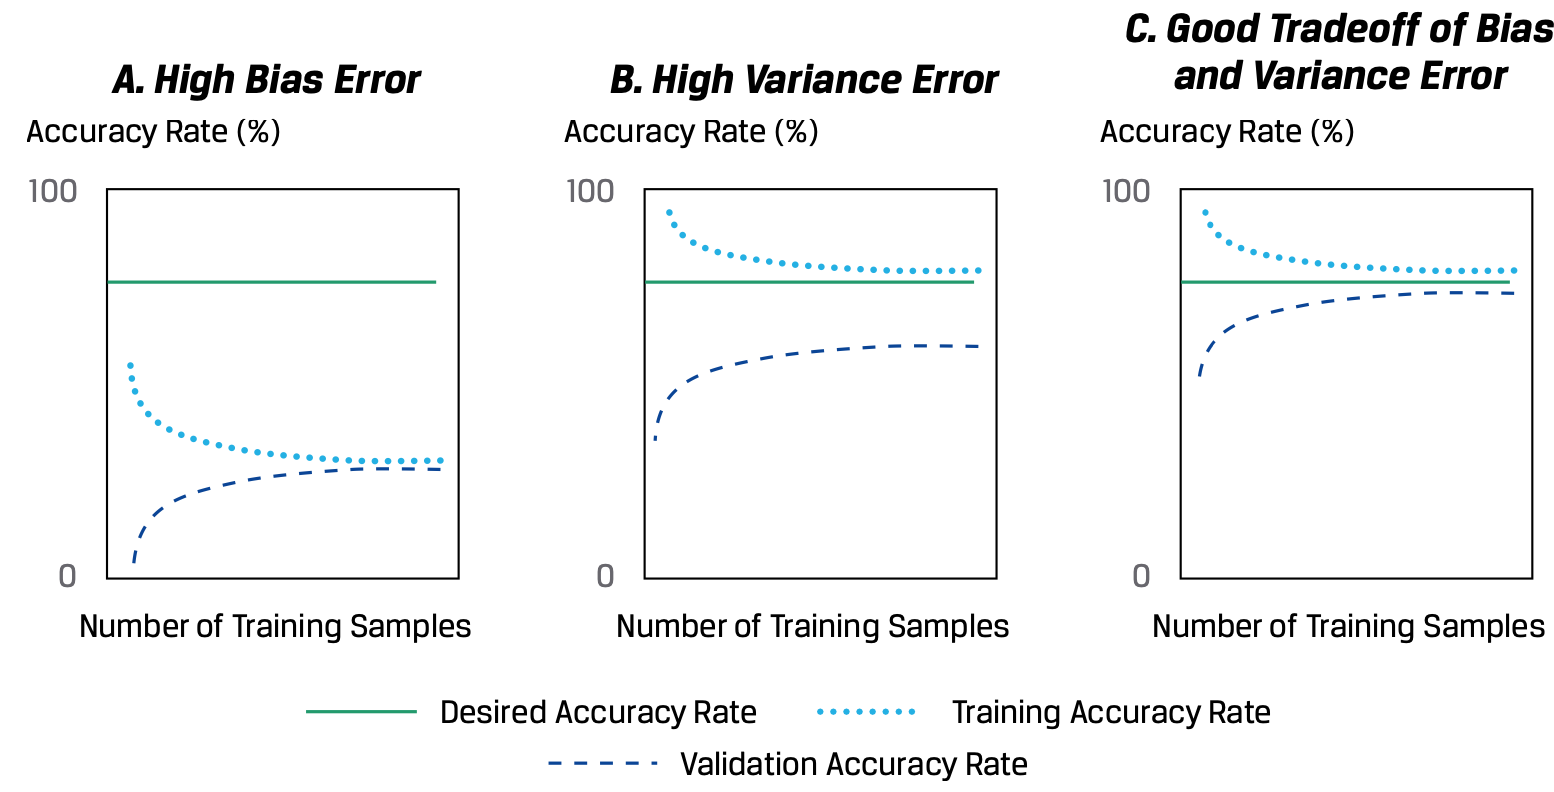
\includegraphics[scale=0.4]{/quant/learningcurves}
\caption{Learning curves showing accuracy in validation and training samples}
\end{figure}

\begin{figure}[H]
\centering
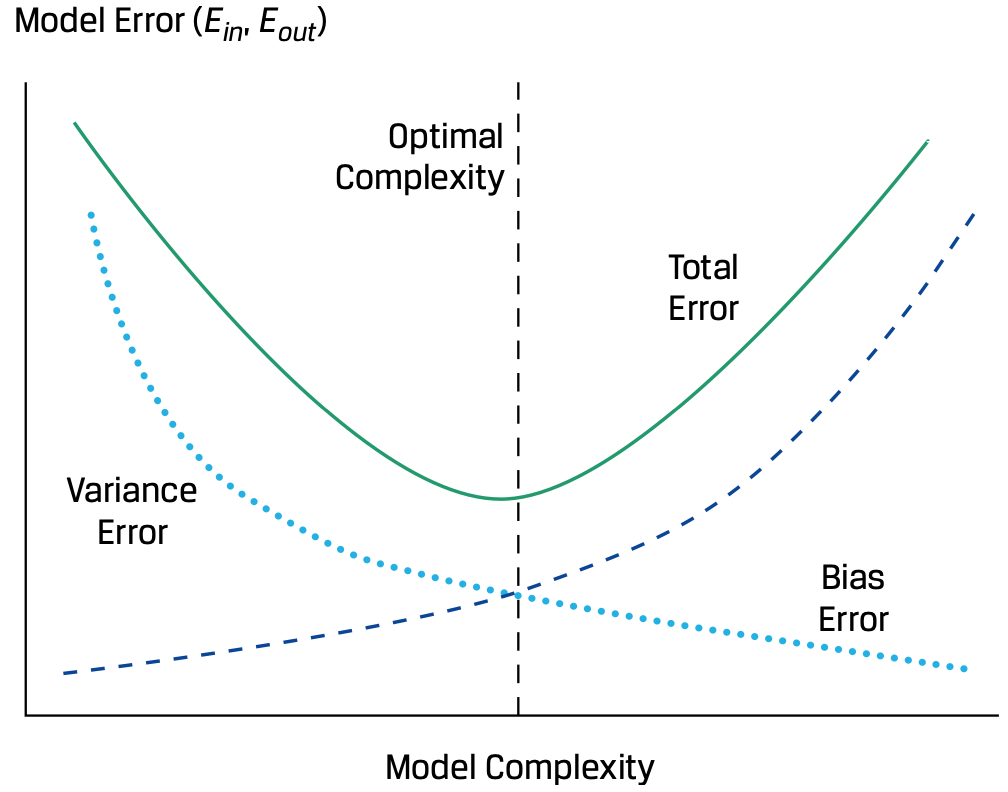
\includegraphics[scale=0.35]{/quant/fittingcurve}
\caption{Fitting curve showing bias-variance tradeoff and model complexity}
\end{figure}

\begin{definition} \hlt{$k$-Fold Cross Validation}\\
Data divided into $k$ samples. Rotate each sample used for validation.\\
Error is then measured for the model in each of the parts, process repeats $k$ times.\\
Average in-sample and out-of-sample error rates are then compiled.
\end{definition}

\begin{definition} \hlt{Penalised Regression}\\
Reduce the problem of overfitting by imposing a penalty based on number of features used.\\
Penalty value increases with number of independent variables used.\\
Penalty exclude features that are not meaningfully contributing to out-of-sample prediction accuracy.\\
Model seek to minimise Sum of Square Errors (SSE) and penalty value. 
\end{definition}

\begin{definition} \hlt{Least Absolute Shrinkage and Selection Operator (LASSO)}\\
In addition to minimising SSE, LASSO minimises the sum of the absolute values of the slope coefficients.\\
LASSO automatically eliminates the least predictive features.
\begin{equation}
\text{Penalty Term} = \lambda \sum\limits_{k=1}^K \abs{\hat{b}_k} \nonumber
\end{equation}
where $\lambda > 0$ is the hyper-parameter that balances between overfitting and parsimonious model.
\end{definition}

\begin{definition} \hlt{Regularisation}\\
Methods that reduce statistical variability in high-dimensional data estimation problems.\\
Aim to reduce regression coefficient estimates toward zero, avoiding complex models and the risk of overfitting
\end{definition}

\begin{definition} \hlt{Support Vector Machine (SVM)}\\
Linear classification algorithm that separates the data into one of two possible classifiers.\\
Algorithm maximises the probability of making a correct prediction by determining the boundary that is farthest away from all the observations, which is a discriminant boundary with margins on the side.\\
Margins are determined by the support vectors, observations that are closest to the boundary.\\
Misclassified observations in training data are handled via soft margin classification. This optimises the tradeoff between a wider margin and classification error.\\
Particularly suited for small to medium-size but complex high-dimensional datasets.
\end{definition}

\begin{figure}[H]
\centering
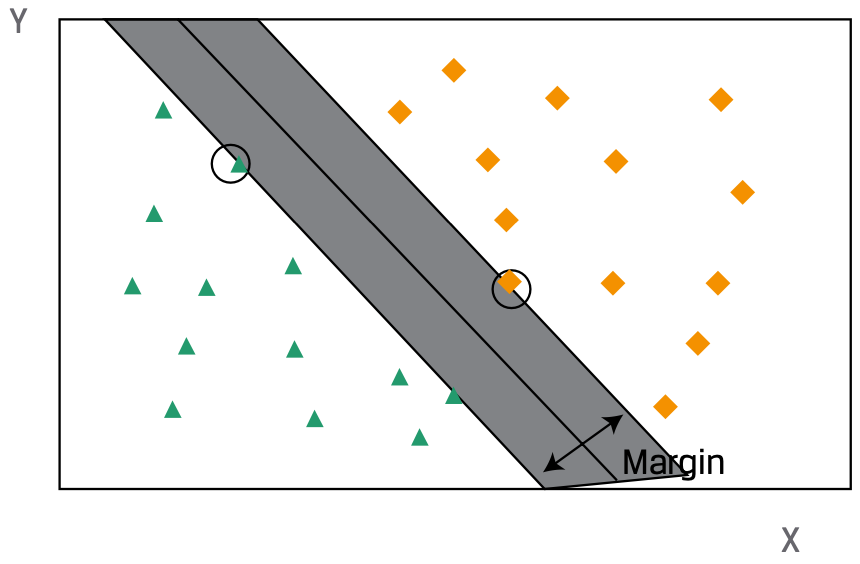
\includegraphics[scale=0.35]{/quant/svm}
\caption{Support Vector Machine}
\end{figure}

\begin{definition} \hlt{$K$-Nearest Neighbour ($K$NN)}\\
Classify an observation based on nearness to the observations in the training sample\\
Hyper-parameter $K$ is specified on number of categories to produce. If $K$ is too small, there is high error rate; if $K$ is too large, result diluted. If $K$ is even, there may be ties, with no clear winner.\\
Requires a distance metric to be specified. Inclusion of irrelevant or correlated features can skew the results.
\end{definition}

\begin{figure}[H]
\centering
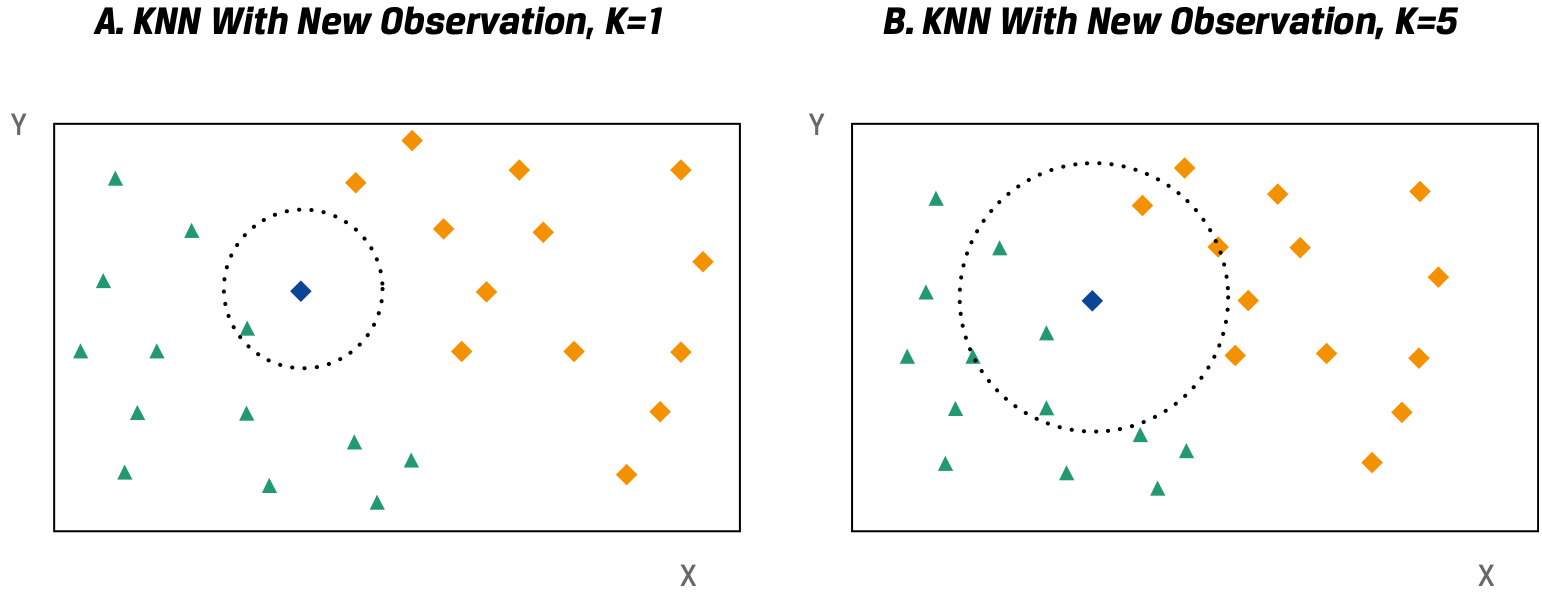
\includegraphics[scale=0.35]{/quant/knn}
\caption{$K$-Nearest Neightbour}
\end{figure}

\begin{definition} \hlt{Classification and Regression Trees (CART)}\\
Appropriate when target variable is categorical, and used when target is binary (classification tree) or a continuous target variable (regression tree).\\
Classification trees assign observations to one of two possible classification at each node. At top of the tree, top feature is selected, and a cutoff value $c$ is estimated.\\
Observations with feature values $> c$ are assigned to one classification, remainder assigned to the other.\\
Tree stops when error cannot be reduced further, resulting in a terminal node.\\
To avoid overfitting, regularisation criteria such as maximum tree depth, maximum number of decision nodes can be specified. Alternatively, sections of tree with minimal explanatory power are pruned.
\end{definition}

\begin{figure}[H]
\centering
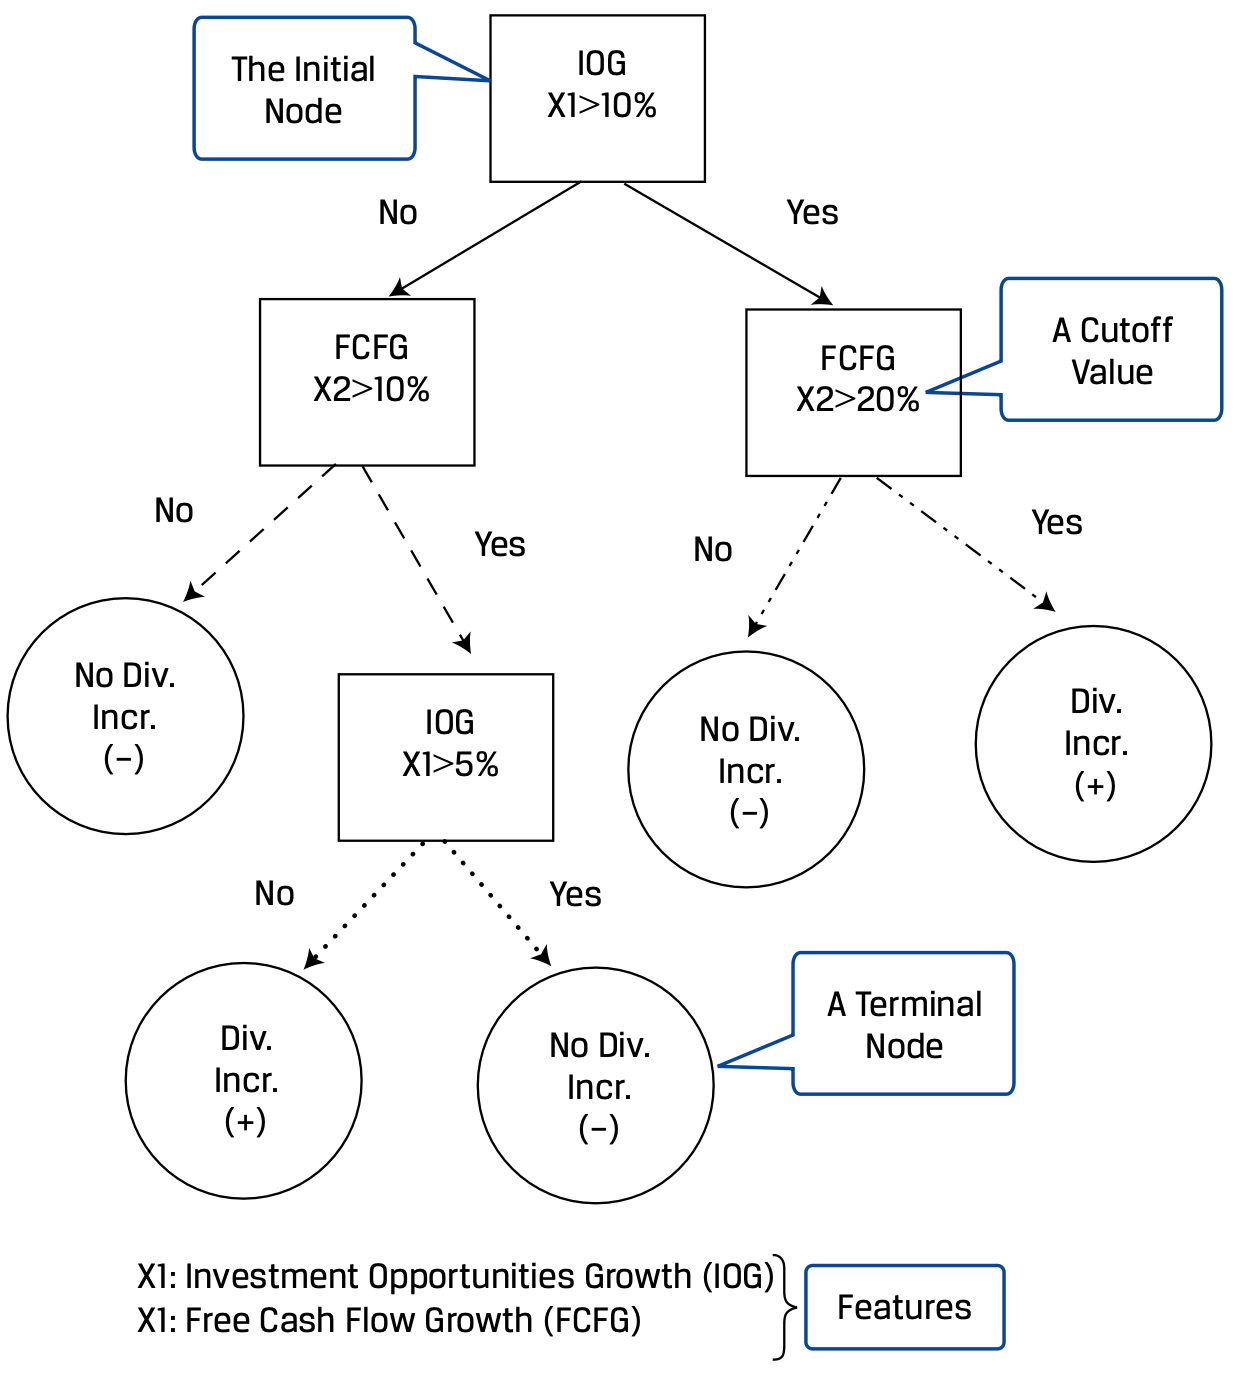
\includegraphics[scale=0.3]{/quant/cart}
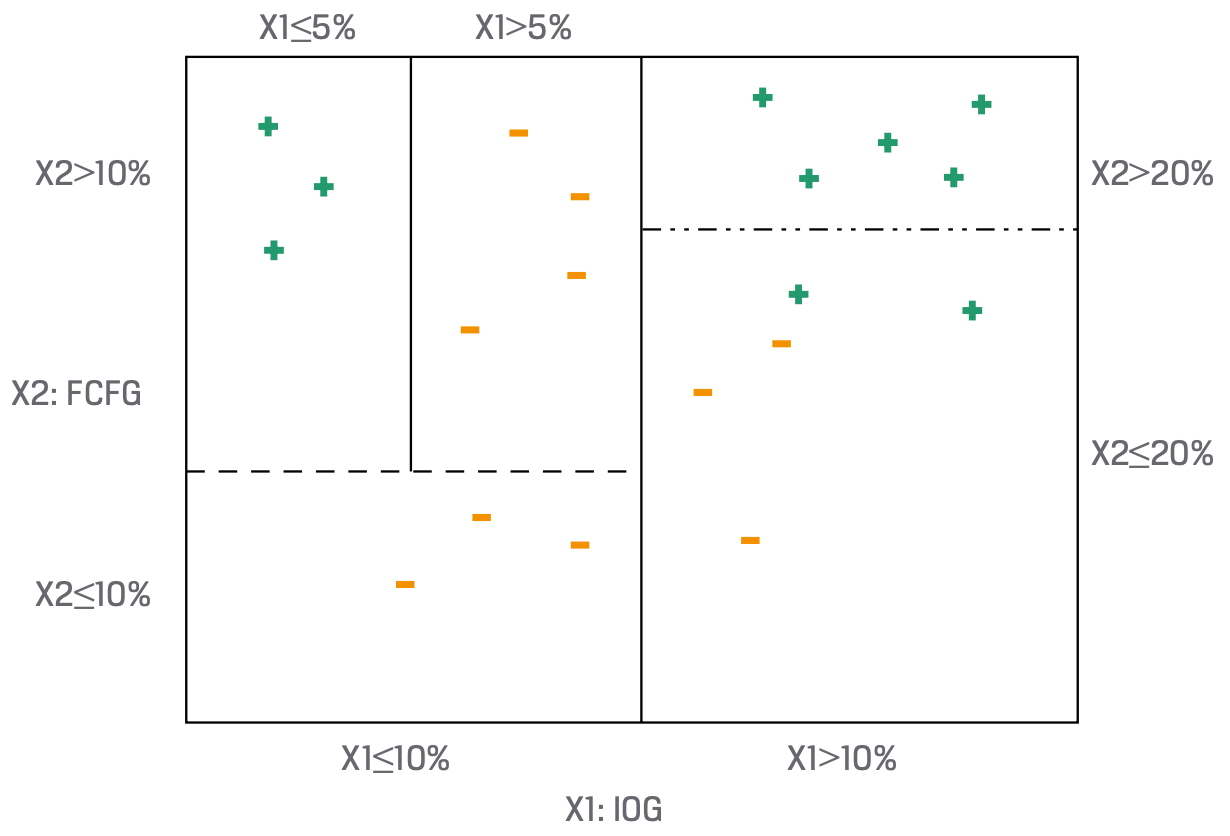
\includegraphics[scale=0.4]{/quant/cartspace}
\caption{CART and the partitioned space}
\end{figure}

\begin{definition} \hlt{Ensemble Learning}\\
Combining the predictions from a collection of models.\\
Produces more accurate and more stable predictions than the best single model. 
\end{definition}

\begin{definition} \hlt{Ensemble Method}\\
Combination of multiple learning algorithms.
\end{definition}

\begin{definition} \hlt{Voting Classifiers}\\
Aggregation of heterogeneous learners, where different algorithms are combined with voting classification.\\
A majority-vote classifier will assign to a new data point the predicted label with the most votes.\\
There is an optimal number of models beyond which performance will deteriorate from overfitting.\\
To look for diversity in the choice of algorithms, modelling techniques, and hypotheses.
\end{definition}

\begin{definition} \hlt{Bootstrap Aggregating (Bagging)}\\
Aggregation of homogeneous learners, where the same algorithm is used on different training data.\\
For each new observation, aggregate the $n$ predictions using a majority-vote classifier for a classification or an average for a regression. Helps to improve the stability of predictions and protects against overfitting the model.
\end{definition}

\begin{definition} \hlt{Random Forest}\\
Collection of a large number of decision trees trained via a bagging method.\\
A randomly selected subset of features is used in creating each tree, which can mitigate the problem of overfitting.\\
Can increase the signal-to-noise ratio because errors across different trees tend to cancel each other out.\\
Note that the transparency of CART is lost when applying random forest classifier.
\end{definition}

\begin{definition} \hlt{Principal Component Analysis (PCA)}\\
Used to summarise or transform highly correlated features of data into a few main, uncorrelated composite variables. Transforms the covariance matrix of features into eigenvectors and eigenvalues.\\
Eigenvectors define new, mutually uncorrelated composite variables that are linear combinations of the original features. Eigenvalue gives proportion of total variance in the initial data that is explained by each eigenvector.
\end{definition}

\begin{definition} \hlt{Scree Plots}\\
Show the proportion of total variance in the data explained by each principal component.\\
The smallest number of principal components that collectively capture $85\%–95\%$ of total variance are retained.
\end{definition}

\begin{figure}[H]
\centering
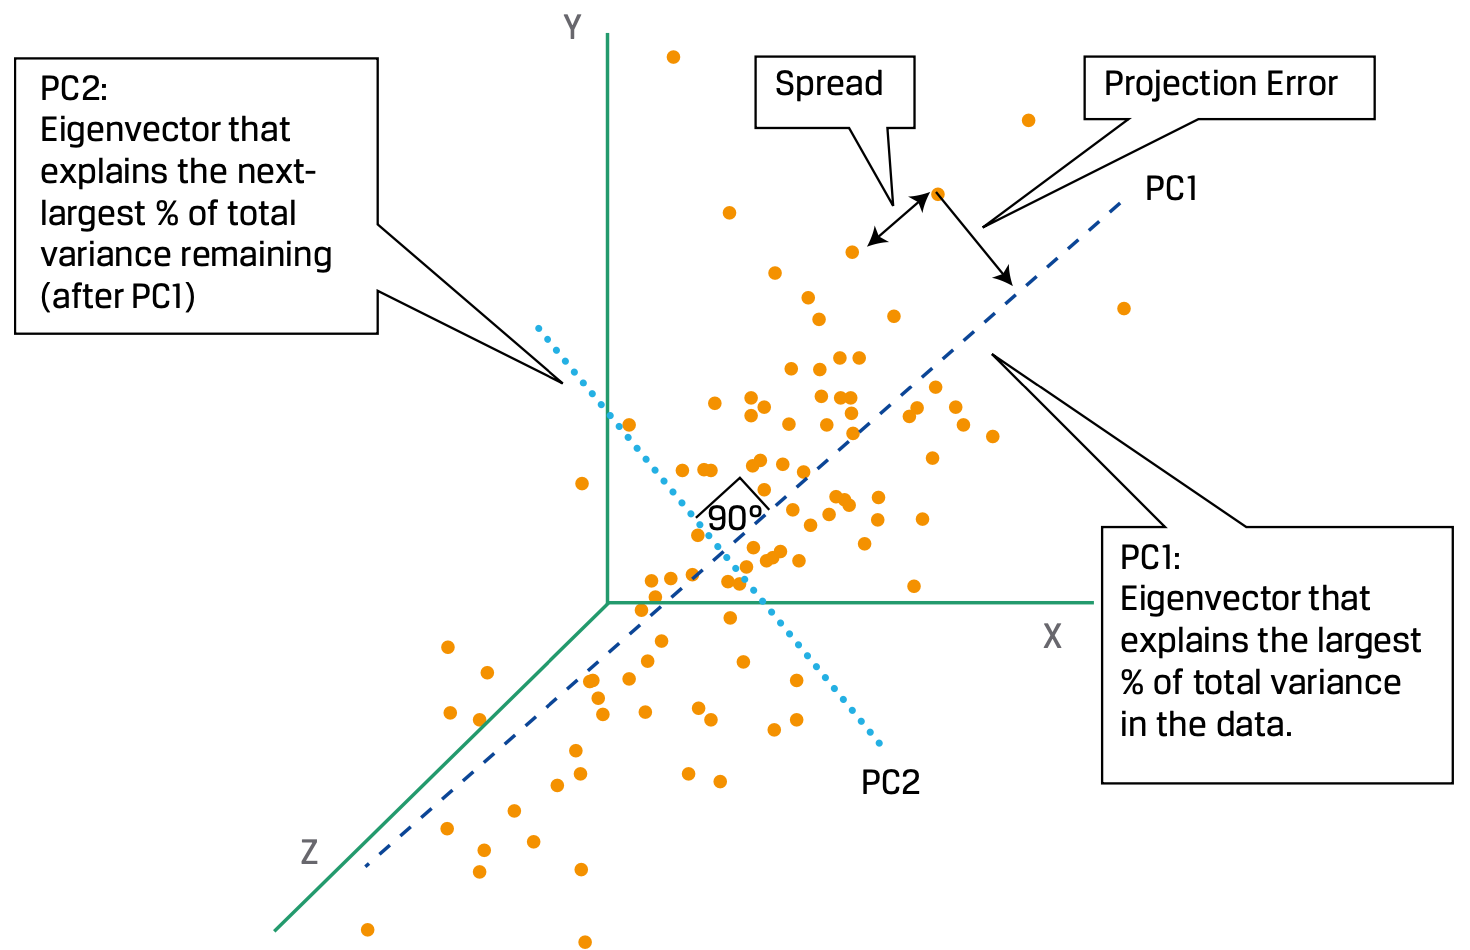
\includegraphics[scale=0.35]{/quant/pca}
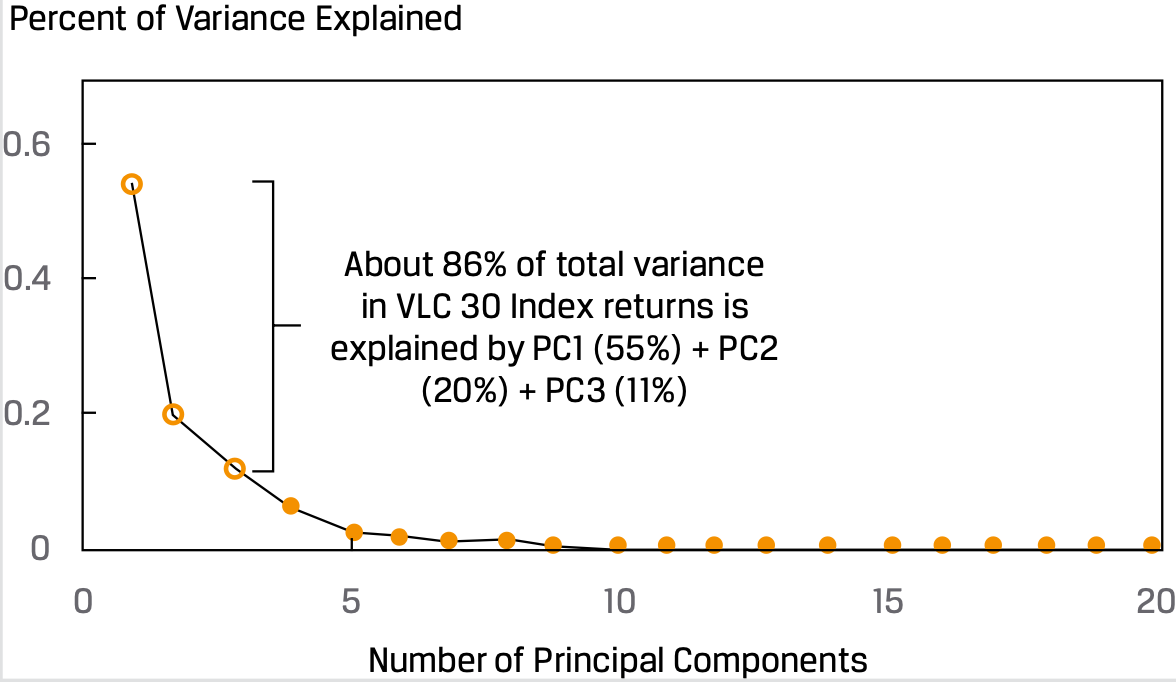
\includegraphics[scale=0.37]{/quant/screeplot}
\caption{PCA and the associated scree plot}
\end{figure}

\begin{definition} \hlt{$K$-Means Clustering}\\
Partitions observations into $k$ non-overlapping clusters, where $k$ is a hyper-parameter.\\
Each cluster has a centroid, each new observation is assigned to a cluster based on its proximity to the centroid.\\
As a new observation gets assigned to a cluster, its centroid is recalculated, which may result in reassignment of some observations, resulting in a new centroid and so forth until all observations are assigned, and no new assignment is made.
\end{definition}

\begin{definition} \hlt{Hierarchical Clustering}\\
Builds a hierarchy of clusters without any predefined number of clusters.\\
May be built bottom-up (agglomerative) or top-down (divisive).\\
Dendrograms may be used to visualise the hierarchical clusters.
\end{definition}

\begin{figure}[H]
\centering
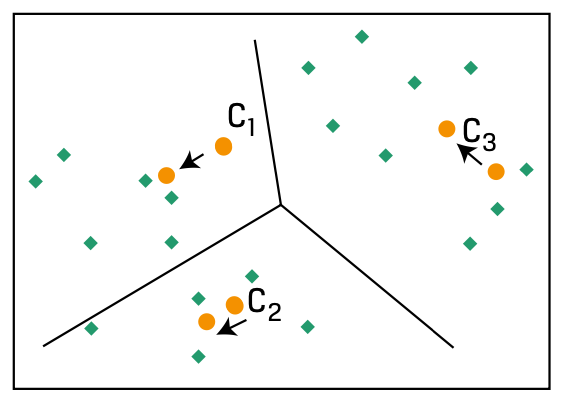
\includegraphics[scale=0.45]{/quant/kmeans}
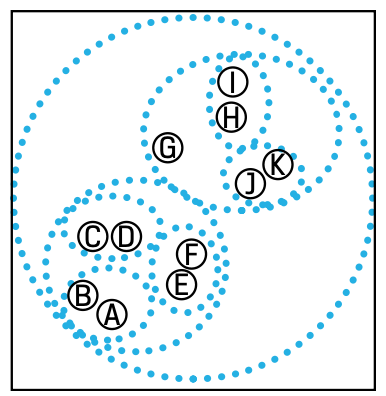
\includegraphics[scale=0.45]{/quant/hcluster}
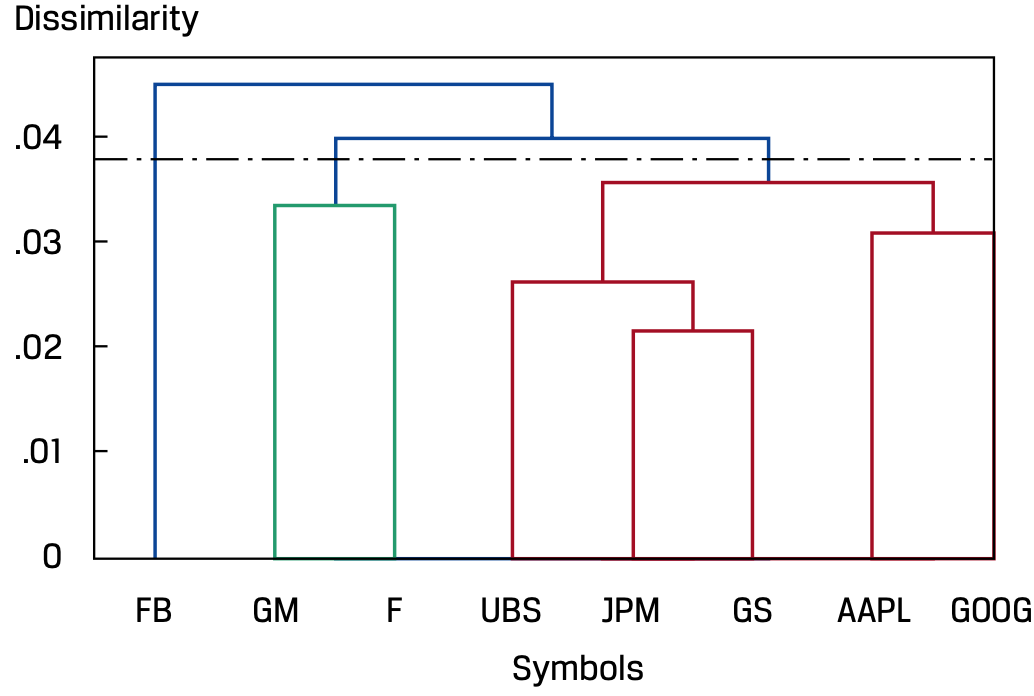
\includegraphics[scale=0.3]{/quant/dendrogram}
\caption{$K$-Means Clustering, Hierarchical Clustering with Dendrogram}
\end{figure}

\begin{definition} \hlt{Neural Networks}\\
Used for classification and regression in supervised learning but are also important in reinforcement learning, which does not require human-labeled training data.\\
Able to model nonlinear relationships between dependent and independent variables.\\
Input layer has nodes equal to dimension (feature set). Hidden layers has nodes with summation operator, activation function. Output layer produces set of probability in target categories. 
\end{definition}

\begin{figure}[H]
\centering
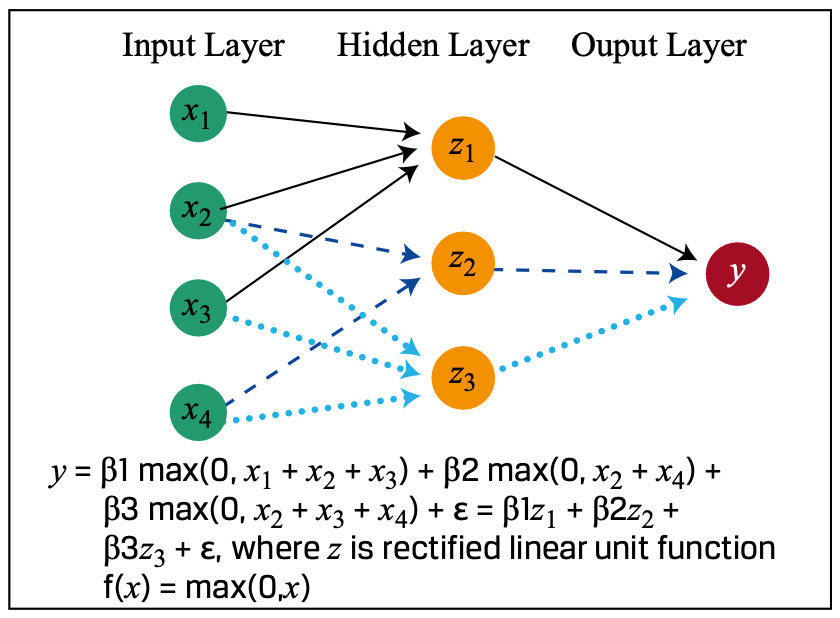
\includegraphics[scale=0.4]{/quant/nn}
\caption{Neural Network}
\end{figure}

\begin{definition} \hlt{Deep Neural Networks (DNNs)}\\
Neural networks with at least $2$ but potentially more than $20$ hidden layers.
\end{definition}

\begin{definition} \hlt{Reinforcement Learning (RL)}\\
Algorithms have an agent that seeks to maximise a defined reward given defined constraints.\\
Does not rely on training data; learns based on feedback from trials. 
\end{definition}

\begin{figure}[H]
\centering
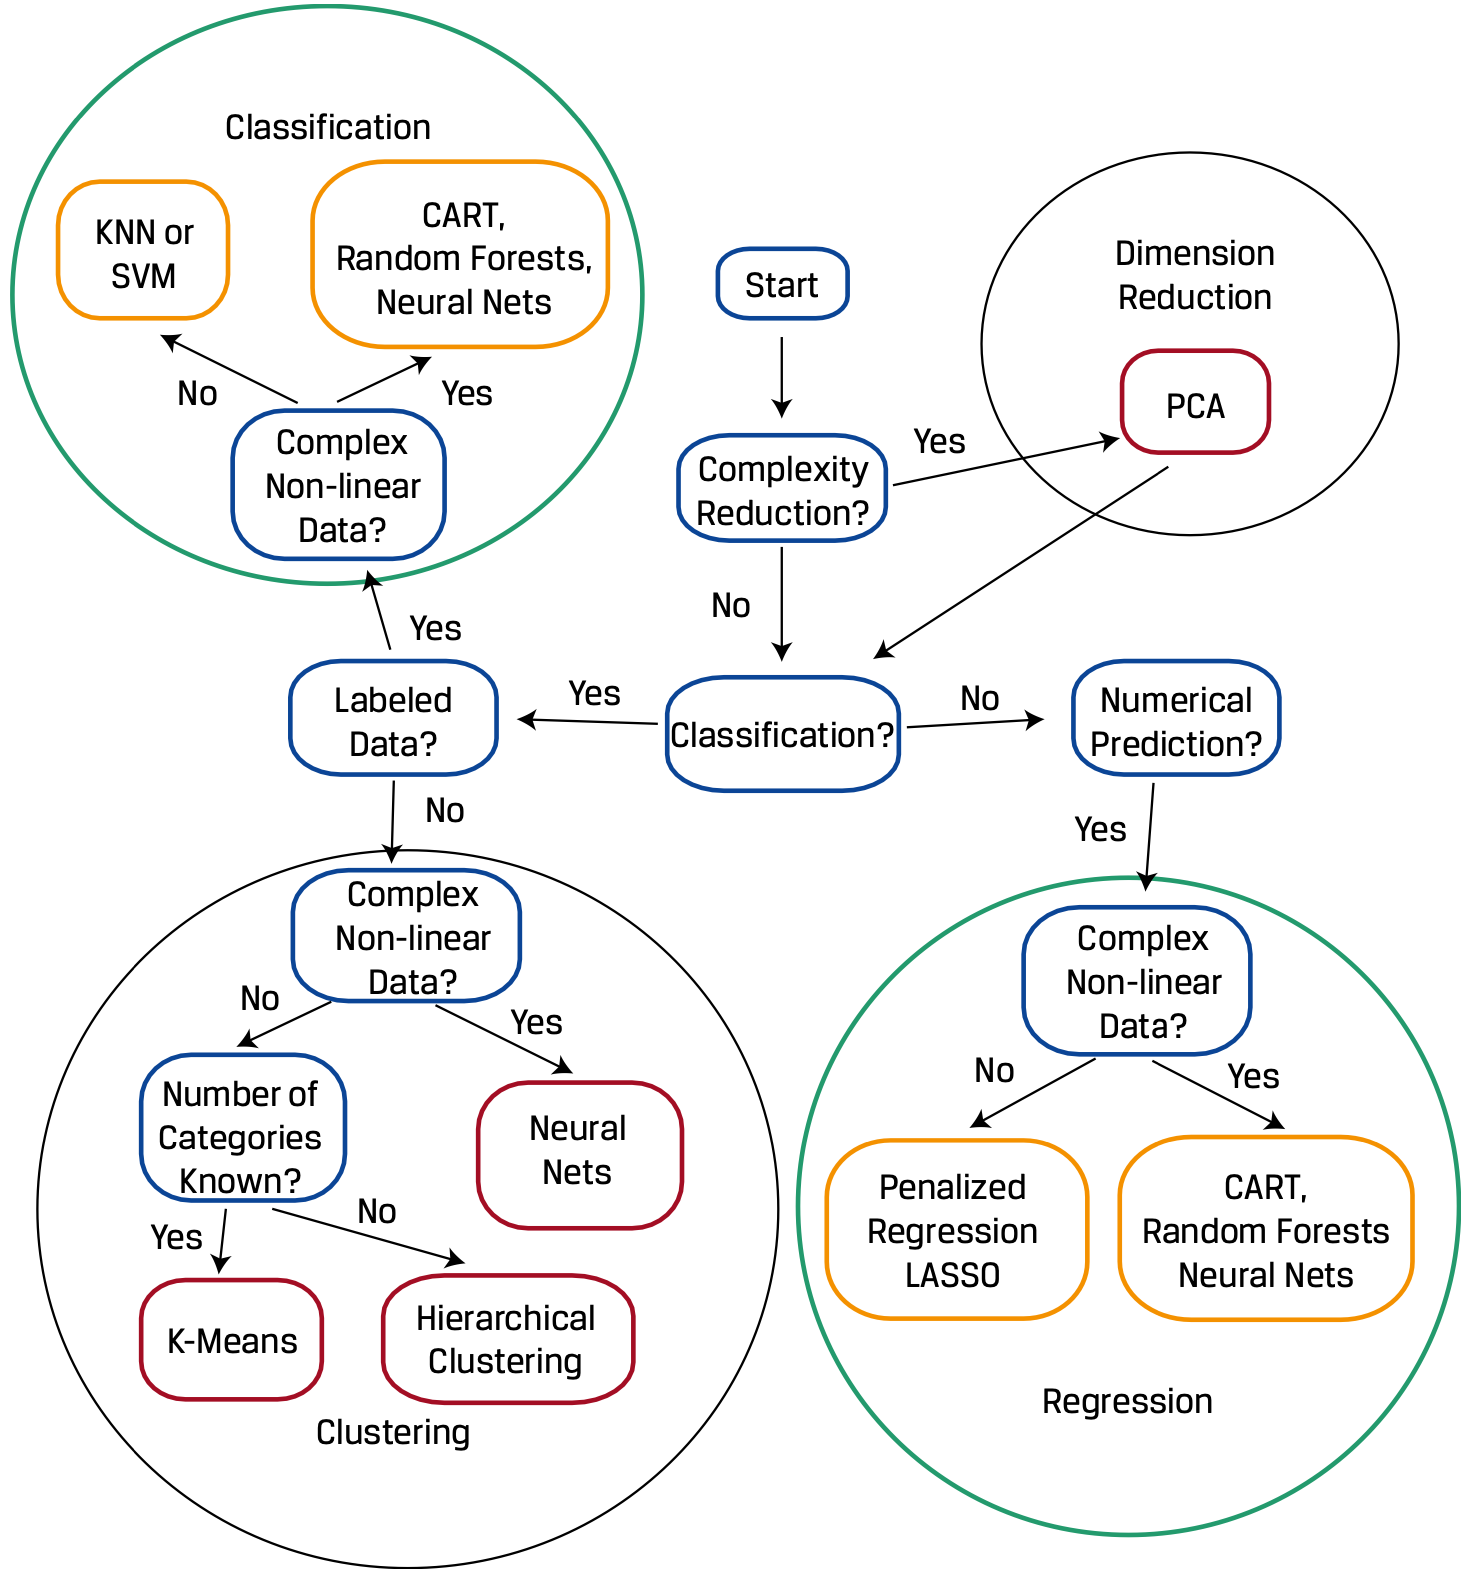
\includegraphics[scale=0.45]{/quant/flowchart}
\caption{Flowchart for choosing ML Algorithms}
\end{figure}
